%! suppress = MathOperatorEscape
%%
%% Copyright 2007, 2008, 2009 Elsevier Ltd
%% 
%% This file is part of the 'Elsarticle Bundle'.
%% ---------------------------------------------
%% 
%% It may be distributed under the conditions of the LaTeX Project Public
%% License, either version 1.2 of this license or (at your option) any
%% later version.  The latest version of this license is in
%%    http://www.latex-project.org/lppl.txt
%% and version 1.2 or later is part of all distributions of LaTeX
%% version 1999/12/01 or later.
%% 
%% The list of all files belonging to the 'Elsarticle Bundle' is
%% given in the file `manifest.txt'.
%% 

%% Template article for Elsevier's document class `elsarticle'
%% with numbered style bibliographic references
%% SP 2008/03/01

\documentclass[preprint,letterpaper]{elsarticle}

%% Use the option review to obtain double line spacing
%% \documentclass[authoryear,preprint,review,12pt]{elsarticle}

%-------- packages --------
\usepackage{amsmath}
\usepackage{amssymb}
%\usepackage{hyperref}
\usepackage{lineno}                 % line numbers
\usepackage[version=4]{mhchem}      % chem formatting
\usepackage{siunitx}                % units formatting
\usepackage{rotating}
%\usepackage{longtable}
%\usepackage{float}
%\usepackage{caption}
%\usepackage{xltabular}
\usepackage{tabularx}
\usepackage{fontawesome}
\usepackage{enumitem}
\usepackage{graphicx}
\setlist{itemsep=0pt}

%-------- package setup --------
\sisetup{exponent-mode = scientific}

%-------- front matter --------
\journal{SoftwareX}

\begin{document}

\begin{frontmatter}

%% Title, authors and addresses

%% use the tnoteref command within \title for footnotes;
%% use the tnotetext command for theassociated footnote;
%% use the fnref command within \author or \address for footnotes;
%% use the fntext command for theassociated footnote;
%% use the corref command within \author for corresponding author footnotes;
%% use the cortext command for theassociated footnote;
%% use the ead command for the email address,
%% and the form \ead[url] for the home page:
%% \title{Title\tnoteref{label1}}
%% \tnotetext[label1]{}
%% \author{Name\corref{cor1}\fnref{label2}}
%% \ead{email address}
%% \ead[url]{home page}
%% \fntext[label2]{}
%% \cortext[cor1]{}
%% \address{Address\fnref{label3}}
%% \fntext[label3]{}

\title{SootLib: a soot model library for combustion CFD}

%% use optional labels to link authors explicitly to addresses:
%% \author[label1,label2]{}
%% \address[label1]{}
%% \address[label2]{}

%\renewcommand{\thefootnote}{\fnsymbol{footnote}}
\author{Victoria B. Stephens}
\author{Josh Bedwell}
\author{David O. Lignell\corref{cor1}}

\cortext[cor1]{Corresponding author \ead{davidlignell@byu.edu}}

\address{Chemical Engineering Department, Brigham Young University, Provo, UT 84602, USA}

\begin{abstract}
sootlib abstract goes here
\end{abstract}

\begin{keyword}
soot \sep combustion \sep reacting flow simulation
\end{keyword}

\end{frontmatter}

\linenumbers

%-------- main text --------

%%%%%%%%%%%%%%%%%%%%%%%%%%%%%%%%%%%%%%%%%%%%%%%%%%%%%%%%%%%%%%%%%%%%%%%%%%%

\section{Introduction}
\label{s:intro}

Most commercial combustion processes that produce energy involve turbulent, non-premixed flames, which produce soot. Soot is responsible for a flame's luminosity, generates a large portion of a flame's radiative heat transfer to its surroundings, and contributes to many of the health, safety, and environmental hazards associated with air pollution from combustion systems~\cite{EPA_2009,EPA_2004}. In order to address soot's negative effects and optimize practical combustion processes, scientists and engineers seek a better understanding of soot's fundamental structure and behavior in combustion environments, often through modeling and simulation.
%Because combustion processes are so complex, modeling and simulation cannot be fully separated from studying fundamental chemical processes; instead, we must use incomplete knowledge and imperfect models to investigate both simultaneously. We often rely on experimental data for comparison, and as a result, errors must be distinguished by their source\textemdash experimental, theoretical, or computational\textemdash which further complicates modeling.
%Turbulent combustion simulation is uniquely challenging because it involves tightly coupled equations of multicomponent mass transfer, convective and radiative heat transfer, turbulent fluid dynamics, multi-phase flow, and complex chemical kinetics.
Combustion processes span many orders of magnitude in both their length and time scales, and simulating soot in flames further expands the range of scales that must be considered, adding additional complexity and computational cost.

Direct simulation approaches can produce accurate simulation data by resolving the full range of length and time scales, but the computational cost can be prohibitively high, particularly for simulating practical combustion processes of interest to engineers~\cite{Pope_2000}.
%High computational cost in combustion simulations is often addressed by modeling various aspects of the configuration.
Computational models that quantify soot production in simulations can help us study its fundamental behavior and distinguish between various reaction mechanisms and transport models while also reducing the potentially high computational cost.
%Reactions involving soot are not purely chemical, but also involve particle aggregation, size distributions, and transport that may or may not affect molecular reactions and heat transfer within a flame.
Accurate models and simulations that help us clarify the fundamental processes that control soot formation and transport in flames represent an important step forward in the study of combustion systems~\cite{Frenklach_2002b}.

SootLib is a convenient, easy-to-use access point for soot property and particle dynamics modeling that can be interfaced with various simulation approaches for combustion CFD.
%SootLib is a modular C++ library that can compute various source terms for the reacting Navier Stokes equations.
SootLib is a C++ library with a modular design that makes model parts interchangeable, allowing users to quickly and easily compare and contrast models within its library of validated mechanisms for soot chemistry and particle dynamics, all of which are implemented with a consistent framework and interface. SootLib provides researchers with convenient access to soot modeling tools suitable for various reacting CFD applications.

%%%%%%%%%%%%%%%%%%%%%%%%%%%%%%%%%%%%%%%%%%%%%%%%%%%%%%%%%%%%%%%%%%%%%%%%%%%

\section{Model Descriptions}
\label{s:models}

Soot models can generally be broken down into two interrelated parts: chemistry and particle dynamics. Soot chemistry models address the chemical reactions involved in soot behavior, including particle inception, growth, and destruction, while particle dynamics models describe the soot particle size distribution (PSD) and its evolution. Given a thermodynamic state and a set of chemical mechanisms, the PSD model predicts changes in the amounts and relative locations of variously sized soot particles based on their current distribution, the desired chemistry, and the thermodynamic state of the surrounding gas. Using a particular set of soot chemistry models generally does not necessitate using a particular PSD model, and vice versa, and SootLib takes advantage of this distinction by allowing users to specify individual models rather than predetermined model sets, giving them more flexibility and control in simulations.

%--------------------------------------------------------------------------
\subsection{Chemistry}
\label{ss:chemistry}

In a modeling context, soot is described as a collection of carbon atoms (though in reality soot may also contain lesser amounts of hydrogen and other elements) above a predefined mass threshold. Soot particles are usually assumed to be spherical, which facilitates calculation of particle diameter, volume, and surface area; this is a reasonable assumption for nascent and relatively small soot particles, but may not be adequate to describe large soot agglomerates, which tend to exhibit fractal structures~\cite{Jullien_1987,Wang_2011}.

Soot chemistry is commonly divided into four primary types: nucleation reactions describe how soot particles form from gaseous precursors, surface growth refers to chemical addition of gaseous species to existing soot particles, oxidation reactions involve soot particle size reduction by reaction with oxygen-based gas species, and coagulation describes how soot particles interact with one another to create new particles. Soot may also undergo additional processes such as growth by condensation of large polycyclic aromatic hydrocarbons (PAH) or agglomeration of particles into large fractal aggregates, but such reactions may or may not be significant in a given scenario. A complete soot chemistry model typically provides a mechanism for all four major steps, each of which occurs independently but depends on the composition and thermodynamic properties of the surrounding gas. Some models provide all four mechanisms, while others expand on earlier mechanisms or focus on one type.

Global kinetic mechanisms, typically represented by Arrhenius-style rate expressions, are popular choices in combustion simulations involving soot, particularly in cases that require soot modeling but cannot afford the relatively high computational cost of detailed soot models or gas mechanisms. Because global models represent each type of soot chemistry with simplified, empirical rate expressions, they do not capture all of the fundamental mechanisms of soot phenomena, but they are relatively simple, easy to implement, and computationally inexpensive. In other words, global models tend to sacrifice accuracy in favor of high speed and low computational cost.
%Additionally, commonly used global models can serve as convenient points of reference when developing or testing modified or more complex soot models.

Physics-based models and mechanisms aim for high accuracy by using multiple elementary reaction steps to represent actual soot behavior rather than relying on the empiricism inherent in global reaction models. By accounting for fundamental phenomena, physics-based models may result in increased accuracy at the expense of computational speed and efficiency. The two-step oxidation models presented below (Section~\ref{sss:oxi}) are simple examples of how using multiple reaction steps can increase accuracy; by accounting for oxidation by both \ce{O2} and \ce{OH}, such models can use validated rate data for elementary reaction steps, potentially resulting in higher accuracy than a model that only considers one oxidation species or combines both dependencies into one empirical rate expression.

SootLib collects a range of models from the literature and implements them with a uniform interface, offering modelers a flexible testing framework and consistent interface for model development and simulations. Table~\ref{t:chem_models} summarizes the soot chemistry models implemented in SootLib.

\begin{sidewaystable}
    \caption{Summary of soot chemistry models implemented in SootLib. In mechanisms, \ce{C(s)} represents a soot particle, i.e. "solid" carbon, and \ce{C(s)^.} indicates a radical site on a soot particle, typically caused by hydrogen abstraction. Variable definitions for rate expressions can be found in~\ref{s:nomenclature}. Rate expressions that involve multiple expressions or otherwise do not fit well in this table can be found in the appendices as noted.}
    \label{t:chem_models}
    \centering
    \resizebox{\textwidth}{!}{
        \begin{tabular}{l l l l l}
            \hline
            Chemistry type  & Model                 & Model ID     & Mechanism & Rate expression \\
            \hline \hline
            Nucleation      & Leung \& Lindstedt~\cite{Leung_1991}  & \texttt{LL}    & \ce{C2H2 -> 2C(s) + H2} & $R_{nuc} = \num{0.1e5} e^{-21100/T} \ce{[C2H2]}$\\
                            & Lindstedt 2005~\cite{Lindstedt_2005}  & \texttt{LIN}   & \ce{C2H2 -> 2C(s) + H2} & $R_{nuc} = \num{0.63e4} e^{-21100/T} \ce{[C2H2]}$\\
                            & PAH nucleation~\cite{Blanquart_2009}  & \texttt{PAH}   & dimerization of gaseous PAH  &\\
            \hline
            Surface growth  & Leung \& Lindstedt~\cite{Leung_1991}  & \texttt{LL}    & \ce{C2H2 + nC(s) ->} (n+2)\ce{C(s) + H2} & $R_{grw} = \num{0.6e4} e^{-21100/T} f(S) \ce{[C2H2]}$\\
                & Lindstedt 1994~\cite{Lindstedt_1994}  & \texttt{LIN}   & \ce{C2H2 + nC(s) ->} (n+2)\ce{C(s) + H2} & $R_{grw} = \num{0.1e-11} e^{-12100/T} \ce{[C2H2]} 2M_0 MW_C$ \\
                & HACA~\cite{Appel_2000,Frenklach_1994} & \texttt{HACA}  & \ce{C(s)-H + H <=> C(s)^. + H2}   & $R_{grw,f}=\num{4.2e13} e^{-13/RT} \ce{[H]}$ \\
                &                                       &                &                                   & $R_{grw,r}=\num{3.9e12} e^{-11/RT} \ce{[H2]}$ \\
                &                                       &                & \ce{C(s)^. + H -> C(s)-H}         & $R_{grw}=\num{2.0e13} \ce{[H]}$ \\
                &                                       &                & \ce{C(s)^. + C2H2 -> C(s)-H + H}  & $R_{grw}=\num{8.0e7} T^{1.56} e^{-3.8/RT} \ce{[C2H2]}$\\
                &                                       &                & \ce{C(s)-H + OH <=> C(s)^. + H2O} & $R_{grw,f}=\num{1e10} T^{0.734} e^{-1.43/RT} \ce{[OH]}$ \\
                &                                       &                &                                   & $R_{grw,r}=\num{3.68e8} T^{1.139} e^{-17.1/RT} \ce{[H2O]}$ \\

            \hline
            Oxidation       & Leung \& Lindstedt~\cite{Leung_1991}   & \texttt{LL}   &  \ce{C(s) + 1/2O2 -> CO} & $R_{oxi,\ce{O2}} = \num{0.1e5} T^{1/2} e^{-19680/T} f(S) \ce{[O2]}$\\
                            & HACA~\cite{Appel_2000,Frenklach_1994} & \texttt{HACA}  & \ce{C(s)^. + O2 -> 2CO + products} & $R_{oxi,\ce{O2}}=\num{2.2e12} e^{-7.5/RT} \ce{[O2]}$\\
                            &                                       &                & \ce{C(s)-H + OH -> CO + products} & $R_{oxi,\ce{OH}}=0.13*1290 P_{\ce{OH}} T^{-1/2} $\\
                            & Lee~\cite{Lee_1962} +
                              Neoh~\cite{Neoh_1980,Neoh_1981}       & \texttt{LEE\textunderscore NEOH} & \ce{C + 1/2O2 -> CO} & $R_{oxi,\ce{O2}} = \num{1.085e4} P_{\ce{O2}} T^{-1/2} e^{-19778.24/T}$\\
                            &                                       &                & \ce{C + OH -> CO + H} & $R_{oxi,\ce{OH}}=0.13*1290 P_{\ce{OH}} T^{-1/2}$ \\
                            & NSC~\cite{Nagle_1962} +
                              Neoh~\cite{Neoh_1980,Neoh_1981}       & \texttt{NSC\textunderscore NEOH} & \ce{C + 1/2O2 -> CO} & see~\ref{a:NSC}\\
                            &                                       &                & \ce{C + OH -> CO + H} & $R_{oxi,\ce{OH}}=0.13*1290 P_{\ce{OH}} T^{-1/2}$\\
            \hline
            Coagulation     & Leung \& Lindstedt~\cite{Leung_1991}  & \texttt{LL}    & \ce{nC(s) -> C_n(s)} & $R_{coa} = -2C_a d_p^{1/2} \left( \frac{6k_B T}{\rho_s}\right) (\rho N)^2$\\
                            & Fuchs~\cite{Fuchs_1964,Seinfeld_2016} & \texttt{FUCHS} & \ce{nC(s) -> C_n(s)} & see~\ref{a:FUCHS} \\
                            & Frenklach~\cite{Frenklach_2002b}       & \texttt{FRENK} & \ce{nC(s) -> C_n(s)} & see~\ref{a:FRENK} \\
            \hline
        \end{tabular}
    }
\end{sidewaystable}

%--------------------------------------------------------------------------
\subsubsection{Nucleation}
\label{sss:nuc}

Particle nucleation refers to the mechanisms by which the smallest possible soot particles are formed. For kinetic-style nucleation mechanisms, SootLib defines a soot particle as a collection of at least 100 carbon atoms, the most common threshold value found in soot modeling literature~\cite{Leung_1991}. Other definitions or threshold values depend on the model used; for example, SootLib's PAH nucleation mechanism defines the smallest possible soot particle as the result of a collision between two PAH dimers~\cite{Blanquart_2009c}. The simplest nucleation models link nucleation rate to the concentration of acetylene (\ce{C2H2}) in the surrounding gas, while more complex models may account for any number of gaseous hydrocarbon species.

SootLib's most basic chemistry model is the simplified kinetic mechanism presented by Leung and Lindstedt (\texttt{LL}), which consists of four Arrhenius-style rate expressions: one each for soot nucleation, surface growth, oxidation, and coagulation~\cite{Leung_1991}. The \texttt{LL} nucleation rate depends only on the concentration of gaseous acetylene and an empirically-determined rate constant. Lindstedt later proposed an alteration to the \texttt{LL} nucleation step's pre-exponential factor to increase accuracy without changing the expression's form (\texttt{LIN})~\cite{Lindstedt_2005}. Both of these mechanisms are known for simplicity and speed rather than accuracy, but may be appropriate under certain conditions.

Experimental literature indicates that soot produced by gaseous fuels tends to nucleate via PAH collisions rather than directly from acetylene precursors, though the precise mechanisms are still unclear~\cite{Wang_2011}. SootLib implements the PAH nucleation model presented by Blanquart and Pitsch (\texttt{PAH}), in which nascent soot particles are created by the collision of two PAH dimers (themselves created by the collision of two PAH molecules)~\cite{Blanquart_2009c}. This model also accounts for condensation of PAH dimers onto existing soot particles, which contributes to chemical surface growth.

%--------------------------------------------------------------------------
\subsubsection{Surface growth}
\label{sss:grw}

Surface growth refers to the addition of carbon atoms to an existing soot particle by reaction with gaseous hydrocarbons. Most soot surface growth models rely on acetylene (\ce{C2H2}) as the primary source of gaseous carbon, though other species may also contribute. Additionally, surface growth models tend to include some dependence on the soot particle's surface area since the availability of sites for the addition of carbon atoms to existing particles tends to be a limiting factor in rate calculations~\cite{Wang_2011}.

The Leung and Lindstedt mechanism for soot surface growth (\texttt{LL}) depends on both the gaseous concentration of acetylene and the particle surface area available for surface reactions. Specifically, it assumes that the number of local active sites available for surface growth and oxidation reactions is proportional to the square root of the total particle surface area in the flame. If the surface area is given by $S=\pi d_p^2 \rho_s N$ and the soot particle diameter by $d_p=(6Y_{s}/\pi \rho_{s} N)^{1/3}$, this surface area dependence becomes
\begin{equation}
    \label{e:surface_area}
    f(S) = \sqrt{\pi \left( \frac{6MW_C}{\pi \rho_{s}} \right) ^{2/3}} \left[ \frac{\rho Y_{s}}{MW_C} \right]^{1/3} [\rho N]^{1/6},
\end{equation}
where $MW_C$ is the molar mass of carbon, $\rho$ is the gas density, $\rho_{s}$ is the solid density of soot, $Y_{s}$ is the mass fraction of soot, and $N$ is the soot particle number density~\cite{Leung_1991}. Lindstedt (\texttt{LIN}) proposed a modified version of the \texttt{LL} surface growth rate that eliminates its dependence on particle surface area in favor of dependence on the particle number density~\cite{Lindstedt_1994}.

The hydrogen-abstraction acetylene-addition (\texttt{HACA}) model presents a more detailed mechanism for both surface growth and oxidation in soot particles. It breaks down the global dependence of surface growth on acetylene into elementary reaction steps with individual Arrhenius-style rate expressions, as listed in Table~\ref{t:chem_models}. Because it is less empirical, the HACA mechanism offers potentially higher accuracy than simpler mechanisms, but its steady-state approach to calculating available soot surface sites keeps its computational cost relatively low~\cite{Appel_2000}. This balance between accuracy and cost makes is a popular choice for modeling soot surface growth and oxidation in combustion simulations.

%--------------------------------------------------------------------------
\subsubsection{Oxidation}
\label{sss:oxi}

Soot oxidation refers to the process by which soot particles lose carbon due to reactions with gaseous species. Similar to surface growth, oxidation mechanisms often depend on the available surface area of oxidizing soot particles, which may or may not be a limiting factor depending on the thermodynamic state, the composition of the gas mixture, and the amount of soot present. Early soot oxidation models tend to rely on \ce{O2} as the principal oxidant, though experimental studies show that \ce{OH} and sometimes \ce{O} can also contribute significantly to soot oxidation rates.

The earliest soot oxidation models depend only on the concentration of gaseous \ce{O2} and one or more empirical rate constants. SootLib implements three such mechanisms: the global rate expression presented by Lee et al.~\cite{Lee_1962}; Nagle and Strickland-Constable's model, in which the oxidation rate depends on a nonlinear combination of Arrhenius-style rate constants~\cite{Nagle_1962}; and the Leung and Lindstedt oxidation expression, which is based on the earlier Lee et al. model~\cite{Leung_1991}.
%The Leung and Lindstedt ({\texttt{LL}}) oxidation model depends only on the concentration of gaseous \ce{O2} and an empirical rate constant. The \texttt{LL} oxidation expression is itself based on an earlier model presented by Lee et al.~\cite{Lee_1962}, which models the oxidation of soot particles by \ce{O2} with a global rate expression. Nagle and Strickland-Constable~\cite{Nagle_1962} also presented a commonly used model for soot oxidation by \ce{O2} in which the rate of oxidation depends on a nonlinear combination of Arrhenius-style rate constants applied to the partial pressure of \ce{O2} (see~\ref{a:NSC}).

These early soot oxidation models, however, do not account for the influence of oxidation by \ce{OH}, which can be significant in certain flame types~\cite{Neoh_1980}. To account for this, SootLib adds expressions for \ce{OH} oxidation presented by Neoh et al.~\cite{Neoh_1981} to the oxidation expressions presented by Lee et al. and Nagle and Strickland-Constable, resulting in the \texttt{LEE\textunderscore NEOH} and \texttt{NSC\textunderscore NEOH} options for soot oxidation in SootLib. Leung and Lindstedt explicitly acknowledge the lack of oxidation by \ce{OH} in their model and consider their one-step oxidation mechanism sufficient for their purposes; in light of their reasoning and the widespread use of the Leung and Linstedt soot model as published, SootLib does not alter or add to the existing Leung and Lindstedt oxidation step.

In addition to the empirical models above, SootLib also includes the HACA mechanism for soot oxidation, introduced in the previous section and detailed in Table~\ref{t:chem_models}~\cite{Appel_2000}. The HACA mechanism accounts for oxidation by both \ce{O2} and \ce{OH} and adds the previously-discussed dependence on particle surface area available for reaction.

%--------------------------------------------------------------------------
\subsubsection{Coagulation}
\label{sss:coa}

Coagulation refers to the process by which soot particles increase in size due to collisions with other soot particles. It is closely related to the soot particle size distribution (PSD), which describes the population of soot particles in terms of size, mass, or number density. While most coagulation processes are not technically chemical reactions, coagulation models are typically structured analogously to the strictly chemical reaction steps and are usually categorized as a type of soot chemistry.

SootLib includes three coagulation mechanisms, all of which interact strongly with the PSD models discussed in Section~\ref{ss:PSD_dynamics}. The simplest coagulation model is that presented by Leung and Lindstedt (\texttt{LL}), which describes particle coagulation with a normal square dependence using an empirical agglomeration rate coefficient~\cite{Leung_1991}.

Physics-based coagulation models represent the coagulation rate of two particles with the expression $R_{coa,12}=K_{12}N_1N_2$, where $N_1$ and $N_2$ are the number density of particles 1 and 2, respectively. $K_{12}$ is coagulation coefficient given by $K_{12}=2\pi (D_{p1}+D_{p2})(D_1+D_2)$, where $D_{p1}$ and $D_{p2}$ are the diameters and $D_1$ and $D_2$ are the Brownian diffusivities of colliding particles 1 and 2, respectively~\cite{Seinfeld_2016}. Particle diffusivity, in turn, depends on the surrounding conditions. In the continuum regime, when the mean free path $\lambda_p$ of a diffusing particle is comparable to or less than its radius ($Kn\ll1$), particle diffusion can be calculated with the Einstein-Stokes relation; in the free-molecular regime, when the mean free path $\lambda_p$ of the particle is much larger than its radius ($Kn\gg1$), particle diffusion is described by kinetic theory. Depending on the external conditions, soot particle coagulation can occur at either limit or anywhere in between, a state referred to as the transition regime.

Fuchs (\texttt{FUCHS}) proposed a generalized coagulation coefficient of the form $K_{12}=2\pi (D_{p1}+D_{p2})(D_1+D_2)\beta$, where $\beta$ is a correction factor that accounts for the kinetic effect of the particle regime (see~\ref{a:FUCHS})~\cite{Fuchs_1964, Seinfeld_2016}. In the continuum and free-molecular limits, the Fuchs form of the coagulation coefficient simplifies to the values calculated from the Einstein-Stokes and kinetic theory expressions, respectively. Frenklach (\texttt{FRENK}) uses a harmonic mean of the continuum and free-molecular values to represent the transition regime, reporting that the approach reproduces results given by the Fuchs form of the coagulation coefficient within about 20\% accuracy~\cite{Frenklach_2002b,Kazakov_1998}.

%--------------------------------------------------------------------------
\subsection{Particle size distribution and dynamics}
\label{ss:PSD_dynamics}

In addition to the chemical reactions that influence their creation and destruction, soot particles also undergo non-chemical changes, typically in the form of coagulation, aggregation, and their inverse processes. As a result, it becomes computationally complex to treat each possible combination of carbon atoms as its own chemical species. Instead, we describe the collection of soot particles as a whole with a particle size distribution (PSD). There are two common approaches to the soot PSD: direct/sectional models and moment methods. Direct methods account for every possible particle size, and sectional methods divide the domain of possible soot particle sizes into discrete ranges based on size or mass; in both cases, the number density of soot particles of each increases or decreases according to defined soot chemistry and mechanisms. The more divisions that are defined in a sectional method, the closer the approximation gets to describing the true distribution (as a direct method would), but the higher the computational cost becomes.

Moment methods, on the other hand, describe the PSD using the statistical moments of the distribution, where the $k^{th}$ mass moment of the discrete soot PSD is defined by
\begin{equation}
    M_k = \sum_{i=1}^{\infty} m_i^k N_i,
\end{equation}
where $m$ is the mass and $N$ is the number density of a given soot particle of size $i$. In most practical applications, only a small number of moments (2--8) is required to describe the full PSD. As a result, moment methods are generally much more numerically efficient than sectional methods. Moment transport equations take the form
\begin{equation}
    \label{e:momTransEq}
    \frac{\partial M_k}{\partial t} + \frac{\partial v_k M_k}{\partial x_k} = -\frac{\partial M_k V_k}{\partial x_k} + S_k,
\end{equation}
where the velocity $v_k$ and the diffusion velocity $V_k$ are assumed to be independent of particle size (which is a reasonable assumption for small soot particles transported mainly by convection and thermophoresis). $S_k$ represents the moment source term, which is comprised of the sum of individual moment source terms for the soot chemistry steps, usually one each for nucleation, surface growth, oxidation, and coagulation. While moment equations are exact, their source terms are unclosed---typically requiring fractional moment values---and further knowledge of the size distribution is required to calculate them. Moment methods differ primarily in their approach to the source term closure problem.

SootLib includes four moment models for calculating the source terms of the moment transport equations, summarized in~\ref{t:psd_models}. Two of the models---\texttt{MONO} and \texttt{LOGN}---are assumed-shape size distribution models in which we assume a particular shape for the soot PSD in order to close the source terms. The two remaining models---\texttt{QMOM} and \texttt{MOMIC}---do not assume a shape for the PSD; instead, they obtain values for the unclosed fractional moments via numerical quadrature and interpolation, respectively. At the time of this writing, SootLib does not include either direct or sectional methods, but its structure is designed to be able to accommodate their addition in future releases.

\begin{table}
    \caption{Summary of soot particle size distribution models implemented in SootLib.}
    \label{t:psd_models}
    \centering
    \resizebox{\textwidth}{!}{
        \begin{tabular}{l l l}
            \hline
            PSD model                                    & Model ID & \# Moments   \\
            \hline
            Assumed monodisperse~\cite{Lignell_2008b}     & \texttt{MONO}  & 2      \\
            Assumed lognormal~\cite{Lignell_2008b}        & \texttt{LOGN}  & 3  \\
            Quadrature method of moments~\cite{McGraw_1997,Marchisio_2013} & \texttt{QMOM}  & 2, 4, 6  \\
            Method of moments with interpolative closure~\cite{Frenklach_2002b} & \texttt{MOMIC} & 3\textendash8  \\
            \hline
        \end{tabular}
    }
\end{table}

%\subsubsection{Monodisperse distribution (\texttt{MONO})}
%\label{sss:mono}

SootLib's simplest PSD closure model is the assumed monodisperse size distribution (\texttt{MONO}), which requires only the first two moments of the soot PSD. These two moments, $M_0$ and $M_1$, correspond to the overall particle number density and mass density of soot particles, respectively, and can be used to define an average particle diameter
\begin{equation}
    d = \left( \frac{6M_1}{\pi \rho_s M_0} \right)^{1/3},
\end{equation}
which allows reaction rates to depend on quantities related to particle size, including particle surface area. Fractional moments are computed via logarithmic interpolation between $M_0$ and $M_1$, closing the moment source terms with relatively simple analytic expressions~\cite{Lignell_2008b}.

Due to its simplicity and ease of use, the \texttt{MONO} model is a popular starting point for soot PSD modeling; it is implemented in SootLib for that reason. Its accuracy may be sufficient for simple flame configurations that produce relatively small soot particles in relatively small quantities. Because this model assumes a uniform shape for the soot PSD, however, it tends to lose accuracy as the distribution of soot particles becomes more varied and complex.

%\subsubsection{Lognormal distribution (\texttt{LOGN})}
%\label{sss:logn}

The assumed lognormal distribution (\texttt{LOGN}) model builds on the simplicity of the \texttt{MONO} model by adding a third mass moment, $M_2$, and assuming that the soot PSD can be described by a lognormal distribution rather than a monodisperse distribution~\cite{Lignell_2008b}. Whole-order moments can be calculated based on predefined parameters for the lognormal distribution in combination with $M_0$, and fractional moments can be calculated from the whole-order moments as
\begin{equation}
    M_k = M_0^{1-\frac{3}{2}k+\frac{1}{2}k^2} M_1^{2k-k^2} M_2^{\frac{1}{2}k^2-\frac{1}{2}k}.
\end{equation}

As with the \texttt{MONO} model, the \texttt{LOGN} model is straightforward and computationally efficient while also increasing the potential for accuracy by assuming a more physically viable shape for the soot PSD. Unfortunately, assuming the distribution's shape still causes the model to lose accuracy as the PSD increases in complexity, though it can be appropriate for cases involving relatively small soot particles that do conform to a roughly lognormal PSD.

%\subsubsection{Quadrature method of moments (\texttt{QMOM})}
%\label{sss:qmom}

Higher accuracy can be obtained by avoiding assuming the shape of the soot PSD, but this requires an alternate approach to closing the moment source terms. The quadrature method of moments (QMOM) does this by applying numerical quadrature to the unknown PSD~\cite{McGraw_1997}. SootLib applies the Wheeler algorithm for moment inversion to calculate the weights and abscissas of the unknown soot PSD~\cite{Marchisio_2013,Wheeler_1974}. For a set of $N$ whole-order moments, resulting in $N/2$ weights $w$ and abscissas $x$ from the inversion algorithm, fractional moments can be calculated with
\begin{equation}
    M_k = \sum_{i=1}^{N/2} w_i x_i^k.
\end{equation}

Avoiding specifying a shape for the soot PSD significantly increases the accuracy of the model, particularly when the distribution increases in complexity, and while this does increase the computational resources required, efficient inversion algorithms and careful implementation can reduce it to acceptable levels.

%\subsubsection{Method of moments with interpolative closure (\texttt{MOMIC})}
%\label{sss:momic}

Like QMOM, the method of moments with interpolative closure (MOMIC) also avoids specifying the shape of the soot PSD, but it closes the moment source terms by interpolating between whole order moments to calculate fractional moments rather than applying any numerical quadrature. This potentially increases its numerical efficiency over quadrature methods while retaining similar levels of accuracy. SootLib implements MOMIC as described by Frenklach~\cite{Frenklach_2002b,Frenklach_1987}, which uses a Lagrange interpolation between logarithms of the  whole-order reduced moments, $\mu_k = M_k/M_0$.

Experimental studies show that the soot PSD is generally bimodal and may be reasonably approximated by the combination of a lognormal distribution and a power law function~\cite{Wang_2011}. It is straightforward to generate an expression for an arbitrary moment based on the distribution parameters, but a nonlinear solver is required to calculate distribution parameters from a given moment set, significantly increasing the time and computational cost of the calculation~\cite{Lignell_2008b}. Additionally, such a distribution still assumes a form for the soot PSD---albeit a more complex one---which restricts its evolution. Under these conditions, it is reasonable to choose methods like QMOM and MOMIC that do not assume a shape for the soot PSD; they can still produce the desired bimodal distribution given a sufficient moment set but have neither the restrictions nor the additional computational overhead of an assumed bimodal distribution. Assumed bimodal distribution models are not typical for these reasons, and, as such, SootLib does not include any models of this type.

%\subsubsection{Sectional model (SECT)}
%\label{sss:sect}

\subsection{Model combinations and limitations}
\label{ss:limitations}

SootLib is designed to be somewhat modular in that the various soot chemistry mechanisms can be substituted and exchanged at will, providing users with increased flexibility. It must be noted, however, that not all model combinations will produce physically meaningful results, either due to a model's design or its author's intent. The following notes indicate possible points of friction and limitations that SootLib users must be aware of when choosing model combinations.

When using SootLib for combustion CFD, the gas-phase chemistry mechanism must include the gas species required by the chosen soot chemistry mechanisms. For instance, a one-step global ethylene mechanism for gas chemistry will generate zero-value source terms for the soot nucleation mechanisms because it does not include the acetylene or gaseous PAH required by SootLib's nucleation mechanisms. SootLib does not explicitly warn users when such situations occur, as there may be cases in which a user finds it advantageous or instructive to exclude or explicitly set a gas species concentration. Therefore, users must take care to choose soot chemistry mechanisms that are appropriate to their use case. One specific model to be aware of in this respect is the \texttt{PAH} nucleation mechanism, which uses the concentrations of a small subset of gaseous PAH molecules. If none of the relevant PAH species is present in the gas mechanism, no soot nucleation will occur. Refer to the SootLib documentation for more details.

The following points apply to individual soot chemistry mechanisms:
\begin{itemize}
    \item The \texttt{LL} model is included with SootLib as a point of reference because it is one of the most common global soot models used in combustion simulations. This model was developed using observations of laboratory-scale ethylene jet flames, and its accuracy and applicability are generally limited to conditions similar to those under which it was developed.
    \item The \texttt{LL} mechanisms were designed to be used together, but can still provide physically meaningful results when separated.
    \item The \texttt{LIN} surface growth mechanism was designed as an improvement to the \texttt{LL} surface growth mechanism and performs most reliably when combined with other \texttt{LL} mechanisms or the \texttt{LIN} nucleation mechanism (which was developed later by the same author).
    \item The \texttt{HACA} surface growth and oxidation mechanisms were not designed to be used separately, but may still perform adequately. Use caution when separating them.
    \item The \texttt{PAH} nucleation mechanism also includes a PAH condensation mechanism. This is by design in order to more closely adhere to the model as presented by its authors~\cite{Blanquart_2009c}. At present, the two cannot be separated, though this may change in future releases.
\end{itemize}

As discussed in Section~\ref{ss:cost}, choosing a soot PSD model for combustion simulations often involves a balance between accuracy and computational cost. While the 2-moment \texttt{MONO} and 3-moment \texttt{LOGN} models are significantly faster than \texttt{QMOM} and \texttt{MOMIC}, they are relatively inflexible because they assume a shape for the soot PSD, limiting its ability to evolve like an actual distribution of soot particles would. That simplicity, however, can be convenient and appropriate for certain applications, such as simulating flames in which soot occurs in relatively small amounts or does not coagulate significantly beyond spherical particles. Methods like QMOM and MOMIC that do not make assumptions about the shape of the soot PSD are advantageous because they allow the soot distribution to evolve naturally, and the number of moments used can be increased to meet accuracy requirements. The more moments that are used to describe the distribution, the more accurately the distribution can be recreated from an arbitrary moment set, but increasing the number of moments can also significantly increase the computational cost of the model.

The following points represent some considerations to make when choosing a soot PSD model for simulations:
\begin{itemize}
    \item Due to the nature of numerical quadrature, \texttt{QMOM} is limited to even-numbered moment sets ($N=2,4,6\ldots$).
    \item A 2-moment QMOM model is functionally equivalent to a monodisperse distribution (MONO), but has additional overhead associated with its implementation. If there is a choice between the two, the \texttt{MONO} model is generally preferable to a 2-moment \texttt{QMOM} model.
    \item For general-purpose soot modeling within combustion simulations, four moments is a good starting point and is generally sufficient to describe a soot PSD for simple gaseous fuels. For more complex fuels or cases requiring higher accuracy, more moments may be required.
    \item Soot particles generally exhibit a bimodal size distribution, which requires five moments to describe accurately. To capture and reproduce this behavior in a simulation, choose a soot modeling approach that uses at least five moments.
%    \item There is no general analytical method for uniquely reconstructing a distribution from its moment set unless the shape of the distribution is known. If such a recreation is required, choose an assumed-size distribution or consider if applicable constraints or assumptions permit use of other tools for reconstructing a distribution from an arbitrary moment set~\cite{Saad_2019}.
\end{itemize}

At present, SootLib does not include any models that account for the agglomeration of soot particles into large aggregates. While it is well known that soot particles tend to form fractal aggregates, simulation of the fractal structure of soot particles is still a relatively young area of research~\cite{Patterson_2007}. Unlike spherical particles, fractal aggregate structures require at least two variables to accurately represent both the size and shape of a particle, and while bivariate PSD models for soot aggregation exist~\cite{Wright_2001,Mueller_2009,Blanquart_2009c}, they tend to be computationally expensive and difficult to implement. SootLib's framework can potentially accommodate multivariate PSD models, making it well-positioned to support this area of active research and development.

%%%%%%%%%%%%%%%%%%%%%%%%%%%%%%%%%%%%%%%%%%%%%%%%%%%%%%%%%%%%%%%%%%%%%%%%%%%

\section{Software description}
\label{s:architecture}

SootLib is an object-oriented C++ library intended for use in combustion CFD codes of various types.
Upon download, the SootLib package contains five directories:
%\begin{itemize}
%    \item[\faFolderO] \texttt{src} contains the SootLib source code;
%    \item[\faFolderO] \texttt{ext} contains externally sourced functions used by SootLib;
%    \item[\faFolderO] \texttt{examples} contains illustrative example codes using SootLib;
%    \item[\faFolderO] \texttt{tests} contains SootLib's optional testing suite, driven by Catch2; and
%    \item[\faFolderO] \texttt{docs} contains the files optionally used to generate code documentation with Doxygen.
%\end{itemize}
SootLib installation is automated by CMake, and project options can be changed by editing the top-level \texttt{CMakeLists.txt} file or, after running the CMake configuration step at least once, by editing the \texttt{CMakeCache.txt} file located in the \texttt{build} directory. Refer to the package documentation for detailed compilation and installation instructions, including the full list of CMake options.
%To build and install the library with the default settings, the user must create and navigate into the \texttt{build} directory and execute the following commands:
%\begin{enumerate}
%    \item \texttt{cmake ..}
%    \item \texttt{make}
%    \item \texttt{make install}
%\end{enumerate}

%Successful installation will generate the following additional directories and files:
%\begin{itemize}
%    \item[\faFolderO] \texttt{include}
%    \begin{itemize}
%        \item[\faFolderO] \texttt{sootlib}
%        \begin{itemize}
%            \item[\faFileTextO] \texttt{constants.h}
%            \item[\faFileTextO] \texttt{sootModel.h}
%            \item[\faFileTextO] \texttt{state.h}
%        \end{itemize}
%    \end{itemize}
%    \item[\faFolderO] \texttt{lib}
%    \begin{itemize}
%        \item[\faFolderO] \texttt{cmake}
%        \begin{itemize}
%            \item[\faFolderO] \texttt{sootlib}
%            \begin{itemize}
%                \item[\faFileCodeO] \texttt{sootlib.cmake}
%            \end{itemize}
%        \end{itemize}
%        \item[\faFileCodeO] \texttt{libsootModel.a}
%    \end{itemize}
%\end{itemize}
To use SootLib in C++ code, include the installed header files---located in the \texttt{include} directory following installation---and link to the \texttt{libsootModel.a} library file. Alternately, SootLib can also be used as part of larger CMake projects via \texttt{sootlib.cmake} (generated during installation) or CMake's FetchContent module.

The SootLib library consists primarily of two object classes through which the user interacts with the library---\texttt{state} and \texttt{sootModel}---both of which are contained within the \texttt{soot} namespace. The \texttt{state} object holds user-specified details about the current thermodynamic state in which the soot chemistry occurs, including variables such as temperature, pressure, and gas species mass fractions. The \texttt{sootModel} object contains information about the selected models and mechanisms and performs the calculations that generate moment source terms. In the context of a traditional CFD simulation, the \texttt{state} object would be updated via the \texttt{setState} function at each time step and/or grid point and followed by a call to \texttt{calcSourceTerms}, whereas the \texttt{sootModel} parameters only need to be specified once when the object is created. The resulting moment source terms, which are calculated assuming that the moment transport equations adhere the form of Equation~\ref{e:momTransEq}, and gas species source terms can be accessed via the \texttt{sootModel} object. For more details on using the SootLib library, refer to the package documentation and examples.

SootLib's major functionalities can be summarized as follows:
\begin{itemize}
    \item Calculates moment source terms (Eq.~\ref{e:momTransEq}) for the soot PSD given thermodynamic state details and chemistry mechanisms chosen by the user; and
    \item Calculates mass fraction source terms for gaseous chemical species affected by soot chemistry, including PAH where appropriate.
\end{itemize}
Auxiliary functionalities and features include the following:
\begin{itemize}
    \item \texttt{str2-SootLibType} functions to facilitate conversion of string values to SootLib's internal enum types for gas species, PAH species, and mechanism specifiers;
    \item Custom \texttt{dimerStruct} structure for access to additional details related to PAH nucleation and condensation calculations; and
    \item Object-oriented, modular mechanism structure designed to facilitate extension to additional mechanisms and model types.
\end{itemize}

%%%%%%%%%%%%%%%%%%%%%%%%%%%%%%%%%%%%%%%%%%%%%%%%%%%%%%%%%%%%%%%%%%%%%%%%%%%

\section{Validation and Examples}
\label{s:examples}

We refer to the literature and the references indicated in Section~\ref{s:models} for the validation of individual models included in Sootlib. Validiating SootLib's implementation of the models with exactness is difficult in the absence of original data, but each model was implemented according to the mathematics presented in the literature and validated against what data was provided (figures, tables, etc.) as best as possible.

Two example scripts are provided to illustrate the main functionality and usage of the SootLib library. The first, \texttt{simpleExample.cc}, is a basic, standalone example of soot model setup, source term calculation, and source term retrieval. This format has limited functionality, but can be useful for directly comparing various models' source term calculations. The second example, \texttt{advancedExample.cc}, illustrates how SootLib might be used in the context of a temporally evolving simulation case. The results of running this example may or may not be physically significant, depending on its inputs; it is primarily intended as an illustration of one potential use case.

%Self preserving size distribution example

%Use simple example code to compare models?

%Validate against literature plots where possible

\subsection{Computational Cost}
\label{ss:cost}

In addition to demonstrating core usage and comparing model attributes, we compared the computational cost of the implemented soot models. Comparisons were performed using a 3.5~\si{GHz} Intel i5-7400 CPU with 8~\si{GB} of available RAM via Windows Subsystem for Linux (WSL). Computational cost is represented by the time required for one thousand evaluations of the \texttt{calcSourceTerms} function averaged over one hundred trials. The base \texttt{sootModel} object used for comparisons was initialized with \texttt{LL} chemistry and a 4-moment \texttt{QMOM} PSD treatment, and the \texttt{state} object represents a stoichiometric ethylene–air mixture, initially at 1 \si{atm} and 298 \si{K}, equilibrated by Cantera at constant pressure and enthalpy.

Figure~\ref{f:cost_chem} summarizes the relative cost of soot chemistry models, where only the model in question differs from the base \texttt{sootModel} object. Results are normalized by the runtime of the base \texttt{sootModel} configuration, which required an average of 0.3156~\si{s} with a standard deviation of \num{6.06E-6}~\si{s}. The results were subjected to a two-tailed Student's T-test, which revealed that the differences in the mean computational time, though small, are significant at a confidence level of 99.9\% for all of the models compared. Despite the statistical significance of the differences in mean computational time for soot chemistry models, these differences may or may not represent a significant addition to the computational cost of a combustion simulation as a whole.

\begin{figure}[ht]
    \caption{Comparison of the computational cost of the soot chemistry models implemented in SootLib. Computational times are normalized by the cost of the base \texttt{sootModel} configuration, which consists of \texttt{LL} chemistry and a 4-moment \texttt{QMOM} PSD treatment.}
    \label{f:cost_chem}
    \centering
    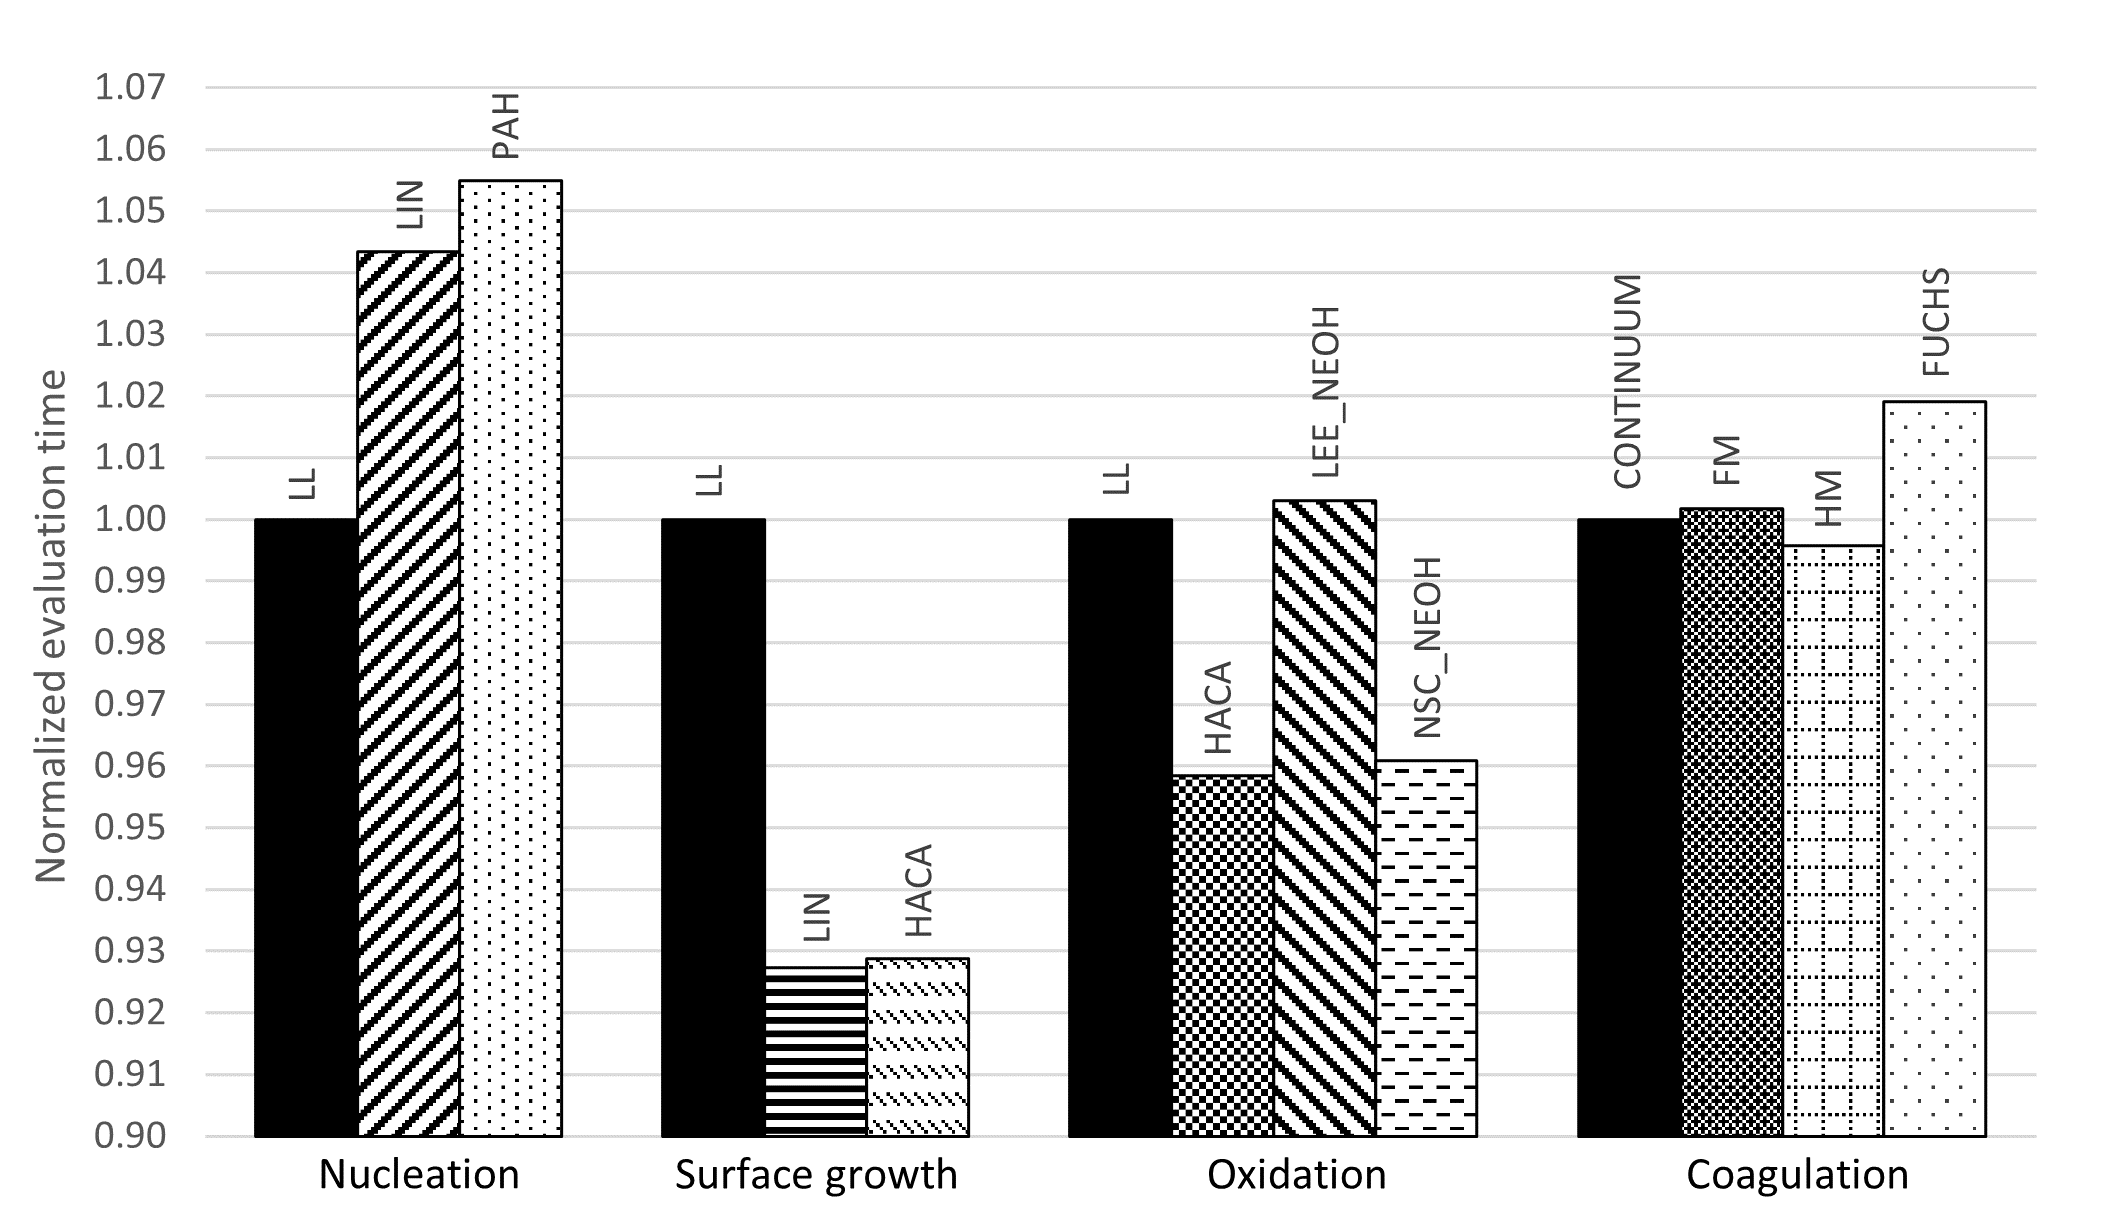
\includegraphics[width=0.85\textwidth]{../figures/comp_cost_chem}
\end{figure}

Figure~\ref{f:cost_PSD} compares the relative computational cost of SootLib's implemented PSD models using the same method and critera as the chemistry comparison, where only the PSD model or the number of moments used differs from the base \texttt{sootModel} configuration. For clarity of presentation, results of the PSD comparison are normalized by the runtime of the 2-moment \texttt{MONO} configuration---which required an average of 0.2961~\si{s} with a standard deviation of \num{5.94E-6}~\si{s}---rather than the 4-moment \texttt{QMOM} configuration used above. A Student's T-test revealed that the differences in mean computational time for PSD models are also significant at a confidence level of 99.9\% for all models compared. The results of the \texttt{MOMIC} configurations are presented on a separate plot (Figure~\ref{f:cost_PSD}b) to highlight the difference in scale compared to the \texttt{MONO}, \texttt{LOGN}, and \texttt{QMOM} models (Figure~\ref{f:cost_PSD}a).

\begin{figure}[ht]
    \caption{Comparison of the computational cost of the soot PSD models implemented in SootLib, including (a) \texttt{MONO}, \texttt{LOGN}, and \texttt{QMOM} (with 2, 4, and 6 moments) and (b) \texttt{MOMIC} (with 3--8 moments). The number above each bar indicates the number of moments used. Results are normalized by the runtime of the \texttt{MONO} configuration with \texttt{LL} chemistry.}
    \label{f:cost_PSD}
    \begin{minipage}{0.5\textwidth}
        \centering
        (a) \\ 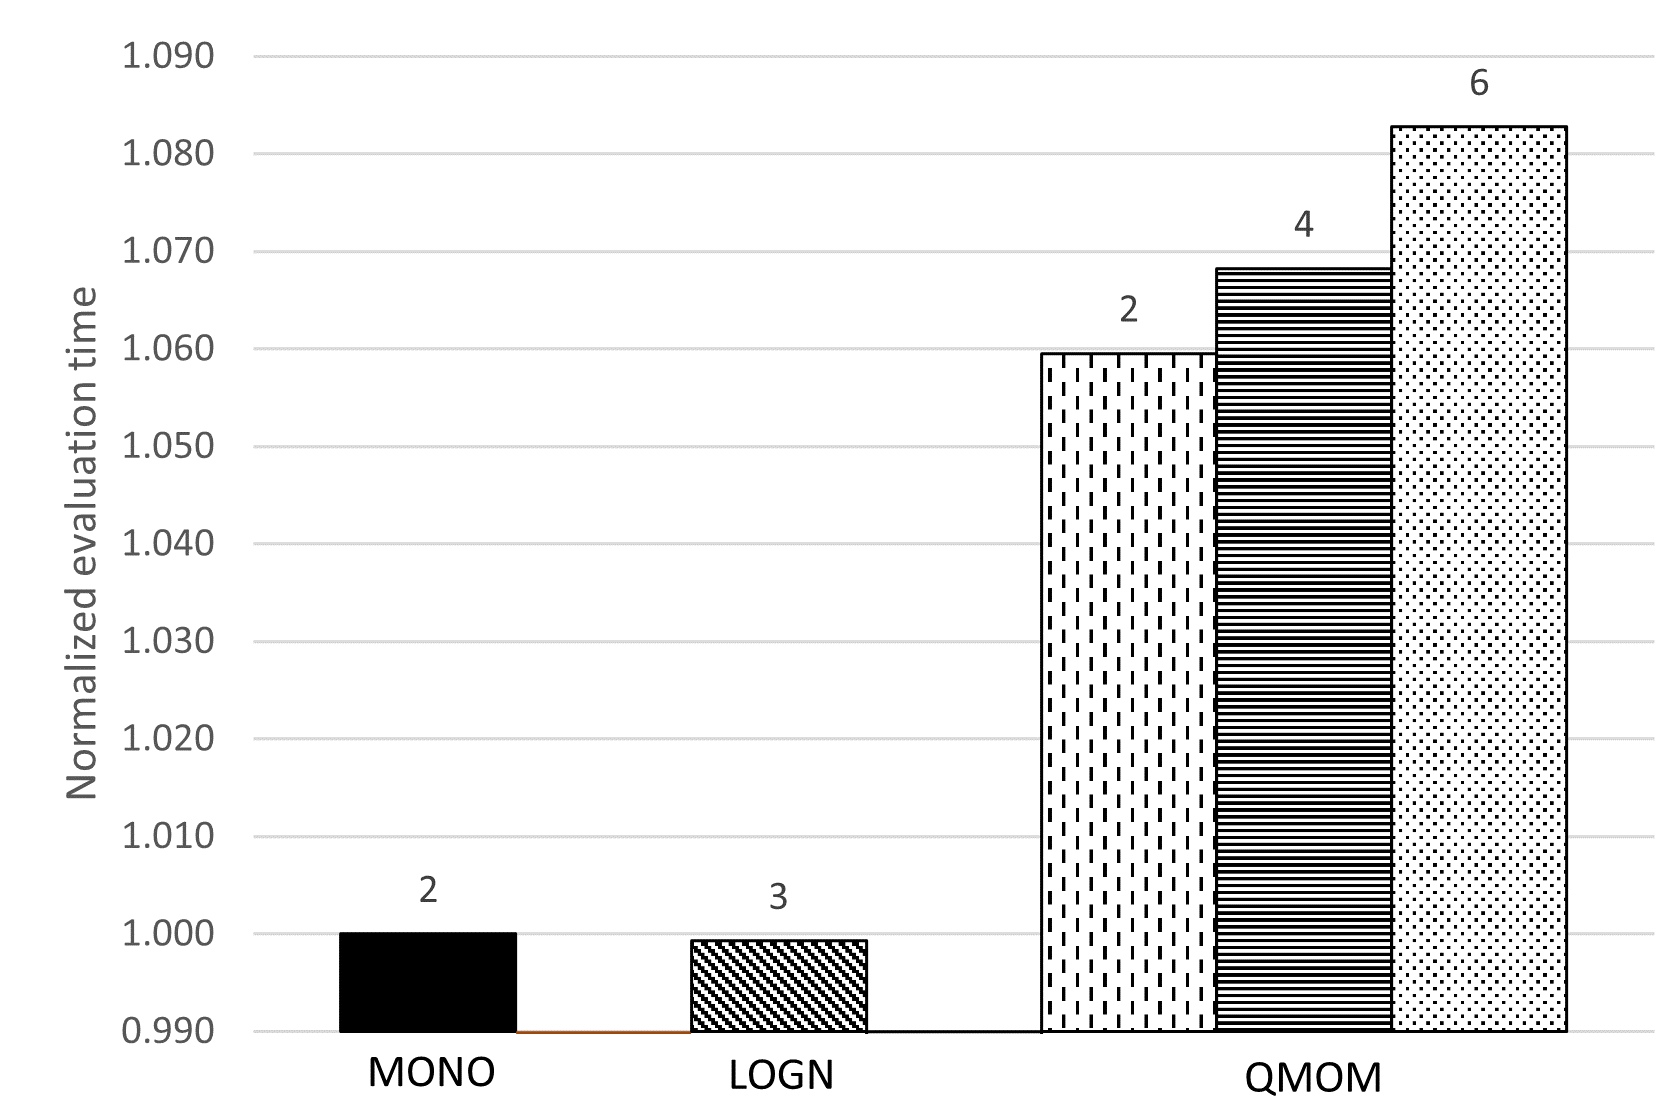
\includegraphics[width=0.9\textwidth]{../figures/comp_cost_PSDa}
    \end{minipage}
    \begin{minipage}{0.5\textwidth}
        \centering
        (b) \\ 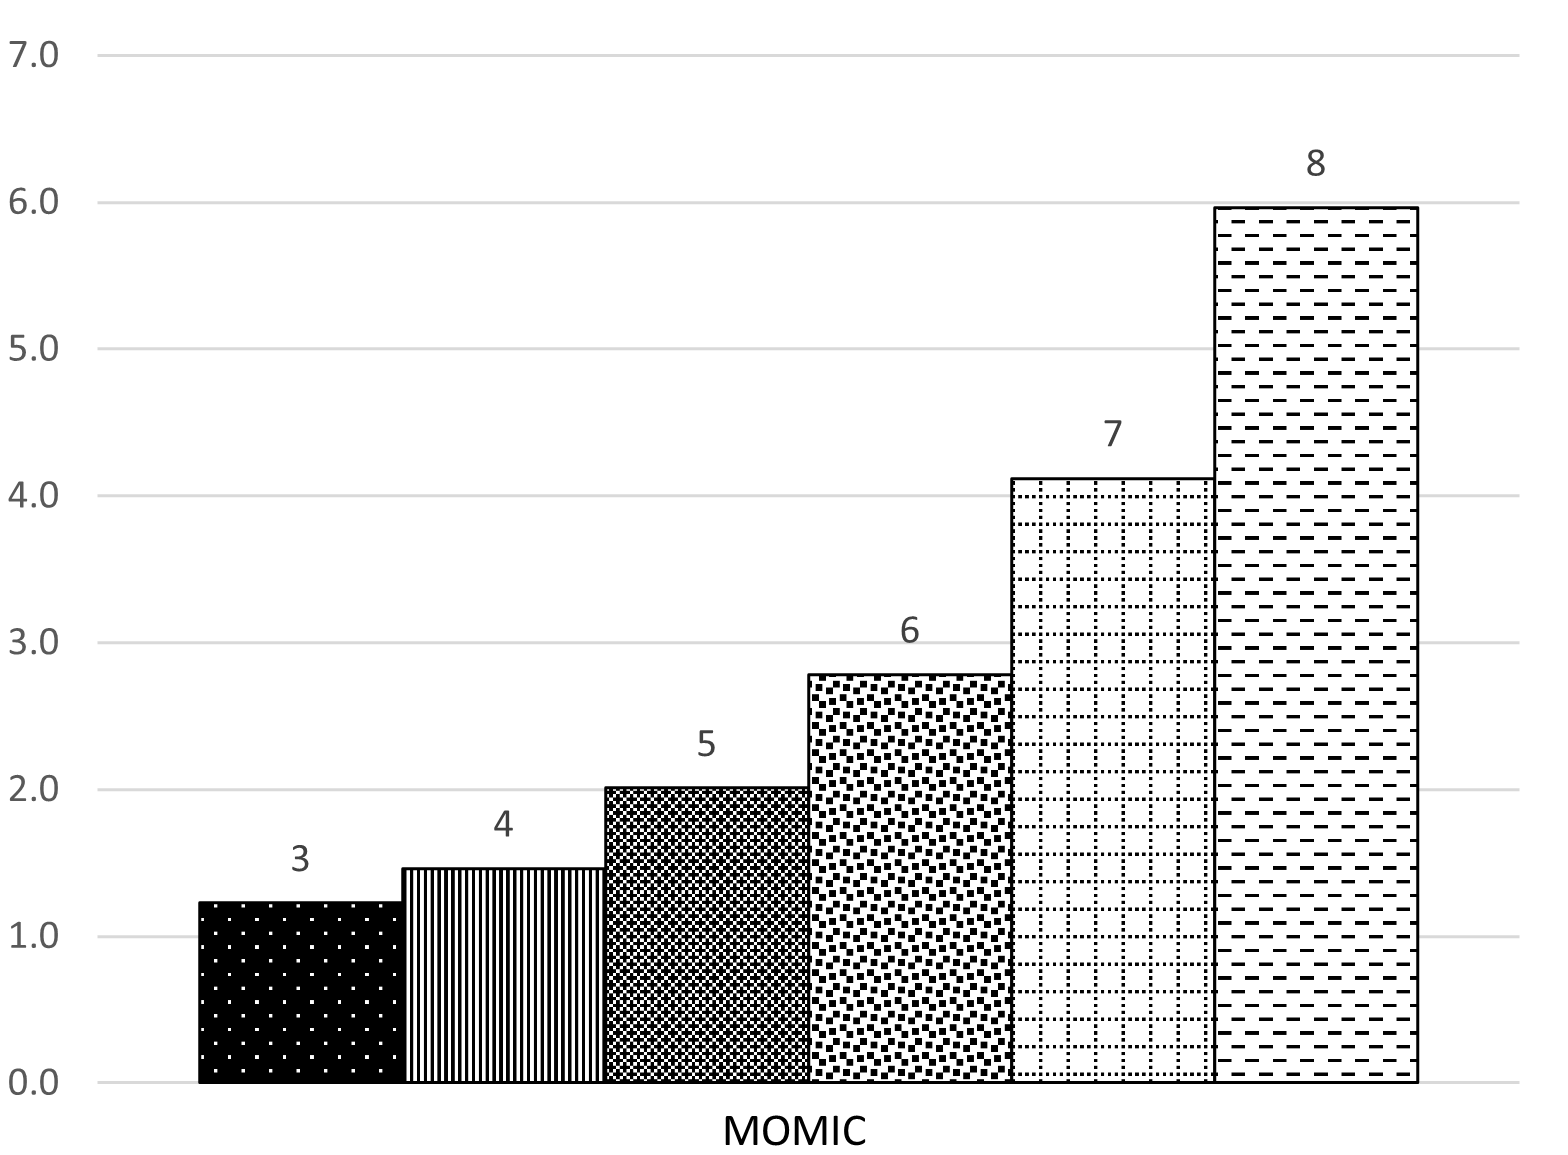
\includegraphics[width=0.9\textwidth]{../figures/comp_cost_PSDb}
    \end{minipage}
\end{figure}

Comparison of Figures~\ref{f:cost_chem} and~\ref{f:cost_PSD} reveals two important points to consider when choosing soot model parameters for combustion simulations. First, the choice of soot chemistry presents much less variation in computational time than the choice of PSD model. That is, choosing a more complex combination of soot chemistry models is unlikely to affect the overall computational cost of a combustion simulation nearly as much as choosing a more complex PSD model would. Second, the choice of PSD treatment and the number of moments to use is non-trivial. As discussed in Section~\ref{ss:limitations}, assuming a shape for the soot PSD (as in the \texttt{MONO} and \texttt{LOGN} models) requires significantly less computational time than more complex methods that do not assume a distribution's shape (such as \texttt{QMOM} and \texttt{MOMIC}), but the time savings comes at the expense of accuracy and flexibility. Thus, choosing an appropriate soot PSD model often becomes a question of balance between accuracy and computational cost.

%%%%%%%%%%%%%%%%%%%%%%%%%%%%%%%%%%%%%%%%%%%%%%%%%%%%%%%%%%%%%%%%%%%%%%%%%%%

\section{Discussion}
\label{s:discussion}

%Indicate in what way new research questions can be pursued as a result of the software (if any).
%
%Indicate in what way, and to what extent, the pursuit of existing research questions is improved (if so).
%
%Indicate in what way the software has changed the daily practice of its users (if so).
%
%Indicate how widespread the use of the software is within and outside the intended user group.
%
%Indicate in what way the software is used in commercial settings and/or how it led to the creation of spin-off companies (if so).

To the authors' best knowledge, there is no existing tool like SootLib, which combines various soot models into one package on a consistent, validated, cross-platform framework that is not specific to any one CFD code or simulation type. SootLib is intended to be a convenient tool that provides combustion CFD researchers with more options and more control over simulations involving sooting flames. For researchers who do not specialize in soot but require soot modeling in order to perform accurate simulations, SootLib lowers the barrier to entry on the topic; it requires a minimum of prior knowledge to use effectively, representing a significant time savings to its users. For combustion researchers who do specialize in soot, SootLib's uniform framework and modular design make it an ideal comparative tool, increasing the potential for useful parametric studies involving soot and decreasing the overhead involved with testing new and existing soot models under a variety of conditions.

At present, SootLib is being used in the authors' research group both independently and as part of the larger development of the one-dimensional turbulence (ODT) model~\cite{Stephens_2021}. When coupled with the RadLib library~\cite{Stephens_2022}, SootLib promises to leverage the low computational cost of the ODT model to perform parametric simulation studies of sooting jet flames that include late-flame soot evolution and soot-flame breakthrough, representing parameter ranges that are typically inaccessible in high-resolution combustion CFD due to excessively high computational cost.

While SootLib was built with combustion CFD in mind, its structure may make it useful in other research areas as well. Topics in atmospheric science and climate change research related to aerosols or carbonaceous particulate matter, for instance, may benefit from SootLib's model library and tools. There is also potential for expansion into areas involving flame methods for materials and nanoparticle synthesis, which share several phenomenological concepts with mechanisms of soot nucleation and behavior~\cite{Wang_2011}.

%%%%%%%%%%%%%%%%%%%%%%%%%%%%%%%%%%%%%%%%%%%%%%%%%%%%%%%%%%%%%%%%%%%%%%%%%%%

\section{Conclusions}
\label{s:conclusions}

SootLib is a C++ library for soot chemistry and particle dynamics modeling, developed for use in combustion simulations and soot model development. Models are implemented on a uniform framework and can be easily interchanged, offering its users flexibility and control in simulation contexts, as well as foundational consistency for model developers. SootLib includes thirteen individual soot chemistry models, including nucleation, surface growth, oxidation, and coagulation processes, and four moment-based models for the soot particle size distribution (PSD), two of which (\texttt{QMOM} and \texttt{MOMIC}) can accommodate a variable number of moments for the soot PSD.

SootLib requires no external dependencies aside from CMake, which handles compilation and installation. The library can be used in C++ projects directly or included in larger CMake projects via its exported package or CMake's FetchContent module.
Users interact with the SootLib library through a small group of objects and functions, contained within the \texttt{soot} namespace, that allow them to specify model parameters, set a thermodynamic state and composition for the gas environment, and calculate source terms for moment transport equations. Two example scripts are provided with the library to illustrate its use.

We demonstrate SootLib's usage through several basic model comparisons, including a comparison of computational cost. In terms of computational cost, the choice of soot PSD model and number of moments impacts the computational time of a given soot model's source term evaluation far more than the choice of soot chemistry. Because SootLib permits flexible combinations of its models, we discuss possible points of friction that may arise from various model combinations and address potential limitations of the implemented models.

SootLib offers advantages to researchers at various levels; for users without a background in soot modeling, SootLib lowers the barrier to entry on the topic by providing validated implementations of popular and effective soot models, while experienced soot modelers can benefit from the consistency of an established framework for implementing and comparing new and existing soot models. In particular, SootLib is well-suited to parametric simulation studies and is currently used in conjunction with the one-dimensional turbulence (ODT) model with an eye toward parametric studies of late-flame soot behavior. While it was developed for combustion simulation research, SootLib is not limited to such use cases, and may also provide support to researchers in other areas that involve carbon-based aerosols such as atmospheric and climate sciences.

%%%%%%%%%%%%%%%%%%%%%%%%%%%%%%%%%%%%%%%%%%%%%%%%%%%%%%%%%%%%%%%%%%%%%%%%%%%

\section{Conflict of Interest}
%Please select the appropriate text:

%Potential conflict of interest exists:
%We wish to draw the attention of the Editor to the following facts, which may be considered as potential conflicts of interest, and to significant financial contributions to this work. The nature of potential conflict of interest is described below: [Describe conflict of interest]

%No conflict of interest exists:
The authors declare that they have no known competing financial interests or personal relationships that could have appeared to influence the work reported in this paper.

%%%%%%%%%%%%%%%%%%%%%%%%%%%%%%%%%%%%%%%%%%%%%%%%%%%%%%%%%%%%%%%%%%%%%%%%%%%

\section*{Acknowledgements}

This research did not receive any specific grant from funding agencies in the public, commercial, or not-for-profit sectors.

%%%%%%%%%%%%%%%%%%%%%%%%%%%%%%%%%%%%%%%%%%%%%%%%%%%%%%%%%%%%%%%%%%%%%%%%%%%

\section*{Nomenclature}
\label{s:nomenclature}

\noindent
{\small
\begin{tabularx}{\textwidth}{l >{\raggedright\arraybackslash}X l}
    \hline
    Variable        & Definition                               & Value \\
    \hline \hline
    $C_a$           & Agglomeration rate constant               & 9.0  \\
    $C_i$           & Cunningham slip correction factor         & \\
    $C_{min}$       & Minimum number of carbon atoms in an incipient soot particle & 100 \\
    $D_i$           & Brownian diffusivity of particle $i$      & \\       % & \si{m^2/s} \\
    $D_{p}$         & Particle diameter                         & \\       % & \si{m} \\
    $K_{ij}$        & Generalized coagulation coefficient       & \\        %& \si{m^3/s} \\
    $Kn$            & Knusden number                            & \\
    $k_B$           & Boltzmann's constant                      & \num{1.3806e-23} \si{J/K} \\
    $M_k$           & k$^{th}$ moment of the particle size distribution & \\  % & \si{kg^k/m^3} \\
    $MW_C$          & Molar mass of carbon                      & 12.011 \si{kg/kmol} \\
    $m_i$           & Mass of particle $i$                      & \\    % & \si{kg} \\
    $N_i$           & Number density of particles of size $i$ (per \si{kg} gas)  & \\   %& \si{\#/kg}\\
    $N_A$           & Avogadro's number                         & \num{6.0221e26} \\
    $P_{i}$         & Partial pressure of gas species $i$       & \\    % & \si{atm} \\
    $R_{coa}$       & Rate of particle coagulation              & \\    % & \si{m^{3}/\# s} \\
    $R_{nuc}$       & Rate of particle nucleation               & \\    % & \si{kmol/m^{3} s} \\
    $R_{grw}$       & Rate of particle surface growth           & \\    % & \si{kmol/m^{2} s} \\
    $R_{oxi}$       & Rate of particle oxidation                & \\    % & \si{kmol/m^{2} s} \\
    $R_{pi}$        & Radius of particle $i$                    & \\    % & \si{kmol/m^{2} s} \\
    $S$             & Particle surface area                     & \\    % & \si{m^2/m^3}-gas \\
    $T$             & Gas temperature                           & \\    % & \si{K} \\
    $Y_s$           & Soot mass fraction                        & \\    % & N/A \\
    $\alpha$             & Coagulation efficiency                    & \\
    $\beta_{c}$         & Continuum regime collision rate function      &  \\ % & \si{m^{3}/\# s} \\
    $\beta_{f}$         & Free-molecular regime collision rate function &  \\ % & \si{m^{3}/\# s} \\
    $\epsilon$             & Van der Waals enhancement factor          & 2.2 \\
    $\lambda_f$           & Gas mean free path                        &  \\ %      & \si{m} \\
    $\lambda_p$           & Particle mean free path                   &  \\ %      & \si{m} \\
    $\mu$             & Gas viscosity                             &  \\ % & \si{kg/m s} \\
    $\rho$             & Gas density                               &   \\ %     & \si{kg/m^3} \\
    $\rho_s$           & Solid soot density                        & 1850 \si{kg/m^3}  \\
    \hline
\end{tabularx}

}

%%%%%%%%%%%%%%%%%%%%%%%%%%%%%%%%%%%%%%%%%%%%%%%%%%%%%%%%%%%%%%%%%%%%%%%%%%%

\appendix

\section{Soot chemistry model rate details}

\subsection{Nagle and Strickland-Constable oxidation rate}
\label{a:NSC}

The rate expression for soot particle oxidation by \ce{O2} presented by Nagle and Strickland-Constable~\cite{Nagle_1962} is
\begin{equation}
    R_{oxi} = \rho_{\ce{C(s)}} \left[ k_A P_{\ce{O2}} \left( \frac{x}{1+k_Z P_{\ce{O2}}}\right) + k_B P_{\ce{O2}} (1-x) \right]
\end{equation}
where
\begin{equation}
    x=\frac{1}{1+\frac{k_T}{k_B P_{\ce{O2}}}}
\end{equation}
and
\begin{equation}
    k_A = 20e^{-15098/T}
\end{equation}
\begin{equation}
    k_B = \num{4.46e-3}e^{-7650/T}
\end{equation}
\begin{equation}
    k_T = \num{1.51e5}e^{-48817/T}
\end{equation}
\begin{equation}
    k_Z = 21.3e^{2063/T}
\end{equation}

\subsection{Fuchs generalized coagulation coefficient}
\label{a:FUCHS}
The Fuchs generalized coagulation coefficient~\cite{Fuchs_1964} for the collision between two particles takes the form $K_{12}=2\pi (D_{p1}+D_{p2})(D_1+D_2)\beta$, where
\begin{equation}
    \beta = \left[ \frac{D_{p1}+D_{p2}}{D_{p1}+D_{p2}+2(g_1^2+g_2^2)^{1/2}} + \frac{8(1/\alpha)(D_1+D_2)}{(\bar{c}_1^2+\bar{c}_2^2)^{1/2}(D_{p1}+D_{p2})} \right]^{-1}
\end{equation}
and 
\begin{align}
    \bar{c}_i &= \left( \frac{8k_B T}{\pi m_i} \right)^{1/2}, \\
    g_i &= \frac{\sqrt{2}}{3D_{pi}l_i} \left[ (D_{pi}+l_i)^3 - (D_{pi}^2+l_i^2)^{3/2} \right] - D_{pi}, \\
    l_i &= \frac{8D_i}{\pi \bar{c}_i}, \\
    D_i &= \frac{k_B T C_i}{3\pi \mu D_{pi}}.
\end{align}
In the continuum limit ($Kn \rightarrow 0$), $\beta=1$ and the generalized coagulation coefficient reduces to
\begin{equation}
    K_{12}=\frac{2k_BT}{3\mu} \frac{(D_{p1}+D_{p2})^2}{D_{p1}D_{p2}}.
\end{equation}
In the free-molecular limit ($Kn \rightarrow \infty)$, the coagulation coefficient can be reduced to
\begin{equation}
    K_{12} = \pi (R_{p1}+R_{p2})^2 (\bar{c}_1^2 + \bar{c}_2^2)^{1/2},
\end{equation}
which is equal to the expression obtained directly from kinetic theory~\cite{Seinfeld_2016}.

\subsection{Frenklach coagulation coefficient}
\label{a:FRENK}

The simplified transition regime model for the coagulation coefficient presented by Frenklach~\cite{Frenklach_2002b} also takes the form $K_{12}=2\pi (D_{p1}+D_{p2})(D_1+D_2)\beta$, but the collision factor $\beta$ is calculated as the harmonic mean of the continuum ($\beta_c$) and free-molecular ($\beta_f$) regime limit values,
\begin{equation}
    \beta = \frac{\beta_f \beta_c}{\beta_f + \beta_c},
\end{equation}
where
\begin{equation}
    \beta_c = \frac{2k_BT}{3 \mu} \left( \frac{C_1}{m_1^{1/3}} + \frac{C_2}{m_2^{1/3}} \right) (m_1^{1/3}+m_2^{1/3}),
\end{equation}
\begin{equation}
    \beta_f = \epsilon \sqrt{\frac{6k_BT}{\rho}} \left( \frac{3\pi \rho}{4} \right)^{1/6} \sqrt{\frac{1}{m_1}+\frac{1}{m_2}} (m_1^{1/3}+m_2^{1/3})^2,
\end{equation}
\begin{equation}
    C_i = 1 + 1.257Kn = 1 + 1.257 \frac{2\lambda_f}{D_i}.
\end{equation}

%%%%%%%%%%%%%%%%%%%%%%%%%%%%%%%%%%%%%%%%%%%%%%%%%%%%%%%%%%%%%%%%%%%%%%%%%%%

%% References:
%% If you have bibdatabase file and want bibtex to generate the
%% bibitems, please use
%%

\bibliographystyle{elsarticle-num}
\bibliography{sootlib-refs}

%% else use the following coding to input the bibitems directly in the
%% TeX file.

%\begin{thebibliography}{00}
%
%%% \bibitem{label}
%%% Text of bibliographic item
%\bibitem{Lignell_2018}
%D.~O. Lignell, V.~B. Lansinger, J.~Medina, M.~Klein, A.~R. Kerstein,
%H.~Schmidt, M.~Fistler, M.~Oevermann, One-dimensional turbulence modeling for
%cylindrical and spherical flows: model formulation and application,
%Theoretical and Computational Fluid Dynamics 32~(4) (2018) 495--520.
%\newblock \href {http://dx.doi.org/10.1007/s00162-018-0465-1}
%{\path{doi:10.1007/s00162-018-0465-1}}.
%
%\end{thebibliography}

%%%%%%%%%%%%%%%%%%%%%%%%%%%%%%%%%%%%%%%%%%%%%%%%%%%%%%%%%%%%%%%%%%%%%%%%%%%

\section*{Required Metadata}

\section*{Current code version}

Ancillary data table required for subversion of the codebase. Kindly replace examples in right column with the correct information about your current code, and leave the left column as it is.

\begin{table}
\begin{tabular}{|l|p{6.5cm}|p{6.5cm}|}
\hline
\textbf{Nr.} & \textbf{Code metadata description} & \textbf{Please fill in this column} \\
\hline
C1 & Current code version & 1.0 \\
\hline
C2 & Permanent link to code/repository used for this code version & https://github.com/byuignite/sootlib \\
\hline
C3  & Permanent link to Reproducible Capsule & \\
\hline
C4 & Legal Code License & MIT \\
\hline
C5 & Code versioning system used & Git \\
\hline
C6 & Software code languages, tools, and services used & C++ \\
\hline
C7 & Compilation requirements, operating environments \& dependencies & C++11, CMake 3.15+, Catch2 (optional) \\
\hline
C8 & If available Link to developer documentation/manual &  \\
\hline
C9 & Support email for questions & davidlignell@byu.edu \\
\hline
\end{tabular}
\caption{Code metadata (mandatory)}
\end{table}

%\section*{Current executable software version}
%
%Ancillary data table required for sub version of the executable software: (x.1, x.2 etc.) kindly replace examples in right column with the correct information about your executables, and leave the left column as it is.
%
%\begin{table}
%\begin{tabular}{|l|p{6.5cm}|p{6.5cm}|}
%\hline
%\textbf{Nr.} & \textbf{(Executable) software metadata description} & \textbf{Please fill in this column} \\
%\hline
%S1 & Current software version & 1.0 \\
%\hline
%S2 & Permanent link to executables of this version  &  \\
%\hline
%S3  & Permanent link to Reproducible Capsule & \\
%\hline
%S4 & Legal Software License & MIT \\
%\hline
%S5 & Computing platforms/Operating Systems & Windows, MacOS, Linux \\
%\hline
%S6 & Installation requirements \& dependencies & C++11, CMake 3.15+, Catch2 (optional)\\
%\hline
%S7 & If available, link to user manual - if formally published include a reference to the publication in the reference list & \\
%\hline
%S8 & Support email for questions & davidlignell@byu.edu \\
%\hline
%\end{tabular}
%\caption{Software metadata (optional)}
%\end{table}

\end{document}
\endinput
%%
%% End of file `SoftwareX_article_template.tex'.